\section{Computer Hardware and Operating Systems}

In the study of techniques used by Ethical Hackers, it is essential to have a thorough understanding of both the components of a computing device and the operating systems. This lesson will explore how a computing device and an operating system function, including the concepts of processes, memory, and the file system.

\subsection{The von Neumann Architecture}
The von Neumann model is a computer architecture proposed by mathematician and logician John von Neumann in the 1940s. This model has been fundamental to the development of modern computers and remains widely used in the design of computing systems.

\subsection{Main Components of a PC/Computing Device}
\subsubsection{Processor (CPU)}
The Central Processing Unit (CPU) is the brain of the computer, responsible for executing software instructions. The primary manufacturers are Intel and AMD.

\subsubsection{Motherboard}
The motherboard connects all the other components of the computer. It contains the main chipset, expansion ports, and connectors for RAM, CPU, and peripherals.

\subsubsection{Memory (RAM)}
Random Access Memory (RAM) is the temporary memory used by the operating system and running programs to store temporary data. RAM is fast but volatile, meaning it loses data when the computer is turned off.

\subsubsection{Storage}
Includes Hard Disk Drives (HDD) or Solid State Drives (SSD). HDDs are cheaper but slower, while SSDs offer higher speeds and no moving parts.

\subsubsection{Graphics Card (GPU)}
Manages graphics and accelerates image rendering. It can be integrated into the motherboard or separate, known as a dedicated graphics card.

\subsubsection{Power Supply Unit (PSU)}
Provides electrical power to the computer. Its power rating must be sufficient to support all components.

\subsubsection{Optical Drive}
Typically a CD/DVD reader or, less commonly, a Blu-ray reader.

\subsubsection{Case}
The enclosure that houses all components. It can come in various sizes and shapes.

\subsubsection{Cooling (Fans and Liquid Cooling)}
Maintains safe temperatures for computer components. Includes CPU and GPU fans, as well as optional liquid cooling systems.

\subsubsection{Network Interface}
Usually integrated into the motherboard, it provides network connectivity such as Ethernet or Wi-Fi.

\subsubsection{Expansion Ports}
USB, HDMI, DisplayPort, audio, and other ports allow the connection of external peripherals such as mice, keyboards, printers, monitors, etc.

\subsubsection{Operating System (OS)}
Software that manages the hardware and provides a user interface for interacting with the computer. Examples include Windows, macOS, and Linux.


\subsection{Binary System and Data Types}
Operating systems process information in binary format, which is a sequence of 0s and 1s. The binary system is a numerical system where all numbers are represented using 0 and 1. Everything handled by a personal computer, such as numbers, characters, and programs, is managed as a sequence of 0s and 1s. The fundamental unit is called a bit (a bit can only be 0 or 1).

Since everything is expressed as a sequence of bits, to describe the nature of the data being processed, an operating system relies on the concept of "data type" which will vary depending on whether the operating system is dealing with a number or a series of characters. The most common data types are shown in the table below:

\begin{table}[h]
\centering
\begin{tabular}{|c|c|}
\hline
\textbf{Data Type} & \textbf{Represents} \\
\hline
\texttt{int} & Used to represent integers \\
\texttt{float} & Used to represent real numbers \\
\texttt{char} & Used to represent characters \\
\texttt{bool} & Used to represent true or false states \\
\hline
\end{tabular}
\caption{Common Data Types}
\label{table:data-types}
\end{table}

\subsection{Logic Gates}
Logic gates are fundamental elements in digital circuit theory and electronic circuit design. They represent fundamental logical operations between boolean inputs (true or false values). Common logic gates include AND, OR, NOT, NAND, NOR, XOR, and XNOR.

\begin{figure}[h]
\centering
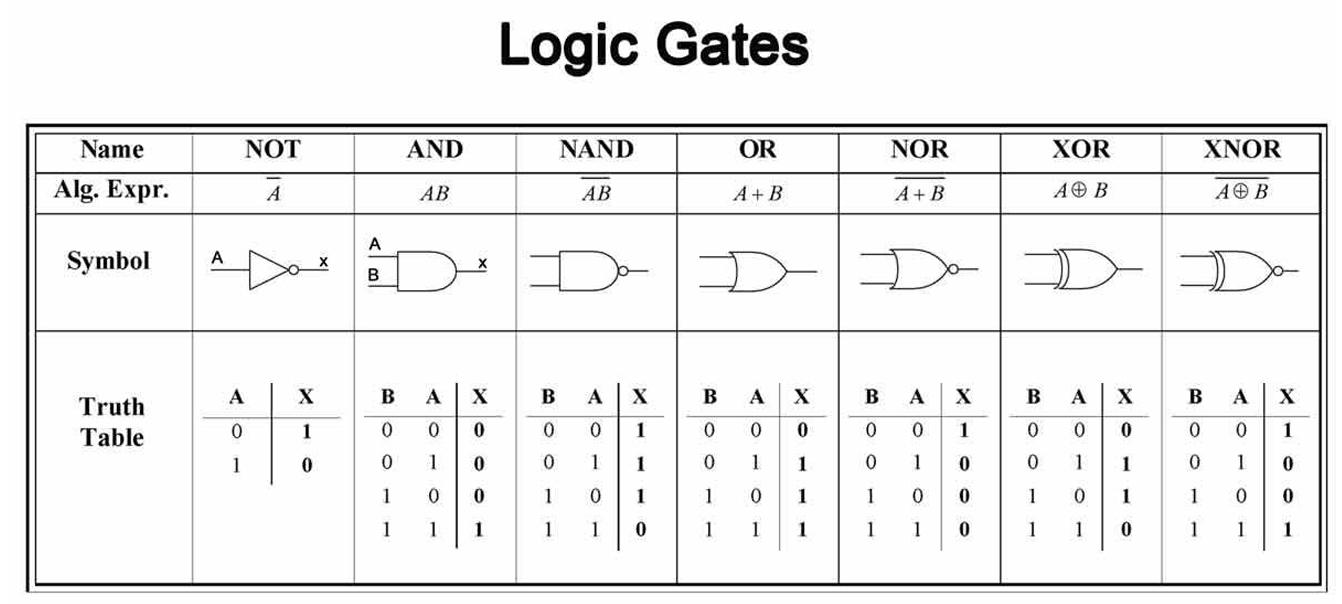
\includegraphics[width=0.8\textwidth]{images/logic_gates.png}
\caption{Logic Gates and Their Truth Tables}
\label{figure:logic-gates}
\end{figure}


\subsection{Operating System Fundamentals}
An operating system (OS) is a crucial software that manages a computer's resources and provides an interface between the hardware and user applications. At its core is the kernel, a critical component that handles low-level operations and directly interacts with the hardware.

\subsubsection{The Kernel}
\begin{itemize}
    \item \textbf{Definition:}
    \begin{itemize}
        \item The kernel is the central and most fundamental part of an operating system.
        \item It is responsible for managing hardware resources, including processors, memory, storage devices, and I/O.
    \end{itemize}
    \item \textbf{Resource Management:}
    \begin{itemize}
        \item Devices: Controls and communicates with hardware devices such as keyboards, mice, and printers.
    \end{itemize}
    \item \textbf{Interaction with Hardware:}
    \begin{itemize}
        \item The kernel provides an abstraction of the hardware, allowing applications to interact with hardware without needing to know the specific details of each device.
    \end{itemize}
\end{itemize}

\subsection{Operating System Functions}
\begin{itemize}
    \item \textbf{System Boot:}
    \begin{itemize}
        \item The boot process begins with the BIOS/UEFI, which loads the kernel into memory.
        \item The kernel starts execution and initiates the operating system's initialization process.
    \end{itemize}
    \item \textbf{Kernel Initialization:}
    \begin{itemize}
        \item During initialization, the kernel configures device drivers.
    \end{itemize}
    \item \textbf{Process Management:}
    \begin{itemize}
        \item When an application is started, the kernel creates a process for it.
        \item The kernel allocates resources and schedules the process to execute instructions on the CPU.
    \end{itemize}
    \item \textbf{Memory Management:}
    \begin{itemize}
        \item The kernel controls memory management.
    \end{itemize}
    \item \textbf{Device Communication:}
    \begin{itemize}
        \item The kernel handles I/O requests, interacting with device drivers to send and receive data to and from devices.
    \end{itemize}
\end{itemize}

\subsubsection{User Interface Interaction}
\begin{itemize}
    \item \textbf{User Interface:}
    \begin{itemize}
        \item The user interface, which can be a Command-Line Interface (CLI) or a Graphical User Interface (GUI), relies on the kernel to perform operations requested by users.
    \end{itemize}
    \item \textbf{Kernel Communication:}
    \begin{itemize}
        \item User applications communicate with the kernel through system calls, requesting specific services such as file reading/writing, memory allocation, etc.
    \end{itemize}
    \item \textbf{Application Management:}
    \begin{itemize}
        \item The kernel manages the execution of applications, ensuring that requested resources are accessed securely and controlled.
    \end{itemize}
\end{itemize}

\subsection{Scenario: System Boot and Application Launch on Windows}
\subsubsection{Phase 1: System Boot}
\begin{itemize}
    \item \textbf{Powering On the Computer:}
    \begin{itemize}
        \item The user powers on the computer with Windows OS installed.
        \item The boot process begins, managed by the bootloader and Windows kernel.
    \end{itemize}
    \item \textbf{Kernel Initialization:}
    \begin{itemize}
        \item The Windows kernel is loaded into memory and starts the initialization process.
        \item Configures device drivers, establishes system settings, and prepares the system for use.
    \end{itemize}
    \item \textbf{Loading the User Interface:}
    \begin{itemize}
        \item The kernel loads the Windows user interface, which may include the desktop and taskbar.
    \end{itemize}
\end{itemize}

\subsubsection{Phase 2: User Interface Interaction}
\begin{itemize}
    \item \textbf{Interacting with the User Interface:}
    \begin{itemize}
        \item The user interacts with the Windows UI, clicking on an application icon in the Start menu or on the desktop.
    \end{itemize}
    \item \textbf{Kernel Request:}
    \begin{itemize}
        \item The user interface sends a request to the Windows kernel to launch the selected application.
    \end{itemize}
    \item \textbf{Process Creation:}
    \begin{itemize}
        \item The Windows kernel creates a new process for the application, allocating resources such as memory and CPU time.
    \end{itemize}
\end{itemize}

\subsubsection{Phase 3: Application Management}
\begin{itemize}
\item \textbf{Application Execution:}
\begin{itemize}
\item The Windows kernel schedules the application’s process to execute on the CPU.
\item The application begins executing its instructions.
\end{itemize}
\item \textbf{Resource Management:}
\begin{itemize}
\item While the application is running, the kernel manages system resources, ensuring the application does not interfere with other processes or misuse resources.
\end{itemize}
\item \textbf{User Interface Communication:}
\begin{itemize}
\item The application communicates with the user interface through the Windows kernel to display output to the user and respond to interactions.
\end{itemize}
\end{itemize}


\subsection{Overview of Kernel Types in Operating Systems}
To reinforce our understanding of key concepts that will be covered in the upcoming slides, we will perform a quick review related to the kernel in general. These topics build a solid foundation for understanding advanced concepts and practical applications of the kernel within our training program.

\subsubsection{Types of Kernels}
There are several types of kernels, each with its unique architecture and functionality. Below are the main types of kernels:
\begin{itemize}
    \item \textbf{Microkernel}:
    A microkernel is a minimalistic kernel that includes only the most essential functionalities of an operating system. An example of a microkernel is \textit{MINIX}. In a microkernel architecture, many services such as device drivers, file systems, and network protocols are implemented in user space, which can lead to better modularity and reliability but may introduce performance overhead due to context switching between user space and kernel space.
    A microkernel, on the other hand, delegates many functionalities to processes in user space, keeping only the essential functions in the kernel itself. This design makes the system more modular and resilient to errors, as components can run in isolated user spaces. However, the communication between components across user-kernel boundaries can slow down performance.
    \item \textbf{Monolithic Kernel}:
    A monolithic kernel is a single binary file that includes most of the functionalities of an operating system. An example of a monolithic kernel is \textit{Unix}. Monolithic kernels run all operating system services in the kernel space, which allows for efficient system calls and better performance. However, this architecture can lead to stability issues, as a failure in one part of the kernel can crash the entire system.
    A monolithic kernel performs most operations directly in the kernel space, including memory management, process management, and communication between system components. This architecture is generally faster because system calls do not need to cross the boundary between user space and kernel space. However, it can lead to stability problems, as a bug in one part of the kernel can affect the entire system.
    \item \textbf{Modular Kernel}:
    A modular kernel can be seen as an extension of the monolithic kernel, with the capability to dynamically add or remove modules as needed. This provides a balance between performance and flexibility, allowing the kernel to be customized for different use cases without requiring a complete recompilation.
    \item \textbf{Hybrid Kernel: The Case of Windows}:
    The Windows kernel is a hybrid kernel, known as the \textit{Hybrid Kernel}. This means it incorporates elements of both monolithic and microkernel architectures.
    The hybrid approach in Windows combines elements of both architectures. For example, certain parts of the kernel, such as memory and process management, are implemented within the kernel itself (monolithic), while other functionalities, such as device drivers, can operate in user space (microkernel-like approach). This hybrid architecture aims to balance the speed of a monolithic kernel with the modularity and stability of a microkernel.
\end{itemize}


The kernel is the core of the operating system, efficiently managing hardware resources and providing a unified interface for user applications. Through precise orchestration of low-level operations, the kernel contributes to providing a stable and secure environment for running programs and interacting with hardware.


\subsection{Overview of Operating Systems}

An operating system (OS) is a software that provides services to users of a computer system and acts as an interface between the user and the physical machine. The primary tasks performed by an operating system include:

\begin{itemize}
    \item Memory management
    \item Process management, where a process is defined as a running program
    \item Process synchronization
    \item User interface management, such as handling input/output (I/O) operations for hardware peripherals like mice, keyboards, and screens
\end{itemize}


\subsubsection{Hardware and Operating System}
Hardware consists of the physical components that make up a personal computer, such as memory (RAM, hard drives, SSDs) and processors (CPUs) that are dedicated to executing instructions. The operating system is responsible for managing these components and providing a stable environment for applications to run.

To handle all these tasks, operating systems are generally composed of multiple modules, each dedicated to a specific function. The operating system organizes the interaction between these different modules, such as:

\begin{itemize}
    \item Process management
    \item I/O management
    \item File system management
    \item Central memory management
    \item User interface
\end{itemize}

\paragraph{Kernel}
The kernel is the core of the operating system, managing interactions between hardware and running processes. The file system is a mechanism that regulates the storage of data on a memory medium in an organized manner.

\section{Process Management}
A process is a running program, and each process is associated with a state, which can be:

\begin{itemize}
    \item \textbf{Running}: The process instructions are being executed by the processor (CPU).
    \item \textbf{Waiting}: The process is waiting for an event to occur (e.g., user input via keyboard).
    \item \textbf{Ready}: The process is waiting to be assigned to a processor to transition to the "Running" state.
    \item \textbf{Terminated}: The process has finished its execution.
\end{itemize}

The process manager module controls the synchronization and state of running programs. In a computer with multiple processes running simultaneously, each CPU executes the instructions of a process for a limited time before switching to another process. This switching of processes in the "Running" state is called scheduling, and the program that determines the time, manner, and sequence of switching is called the scheduler.

In modern multi-CPU systems, the process manager also handles the cooperation between different CPUs. Scheduling can be categorized into two types:

\begin{itemize}
    \item \textbf{Preemptive Scheduling}: The CPU currently in use by a process can be reassigned to execute another process at any time.
    \item \textbf{Cooperative Scheduling}: Once a process is in the "Running" state, it cannot be interrupted until it completes its work and voluntarily releases the CPU.
\end{itemize}

\subsection{Monotasking vs. Multitasking}
Monotasking operating systems can run only one program at a time. In such systems, the execution of a program cannot be suspended to assign the CPU to another program. These systems are generally outdated (e.g., MS-DOS). Monotasking systems are inefficient due to frequent periods of CPU idleness, as shown in the following graph:

\begin{figure}[h]
    \centering
    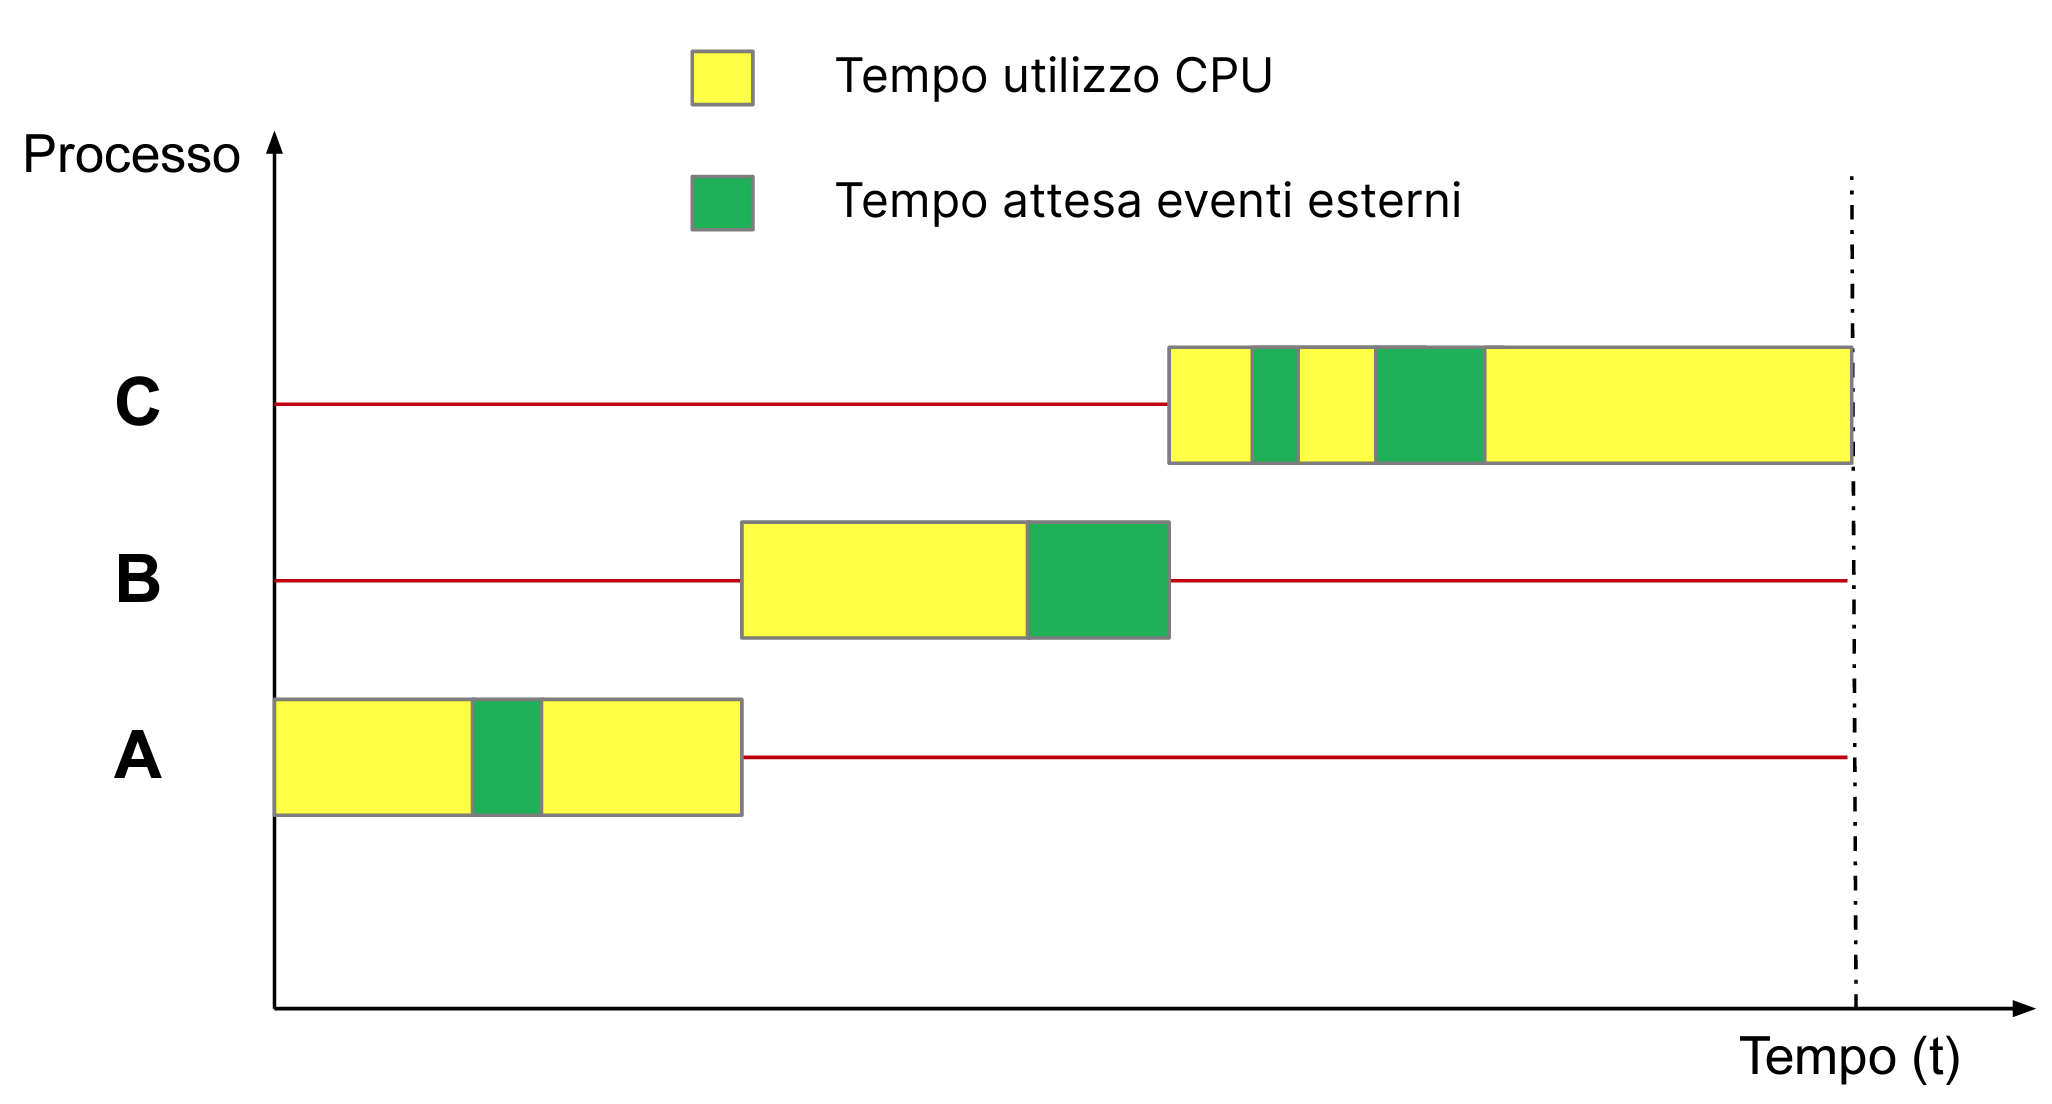
\includegraphics[width=0.8\textwidth]{images/monotask.png}
    \caption{Inefficiency of Monotasking Systems}
    \label{fig:monotasking_inefficiency}
\end{figure}

Multitasking operating systems allow the concurrent execution of multiple programs. Examples of multitasking operating systems include Windows-NT and Linux-based systems. In multitasking systems, processes can be interrupted to shift the CPU's attention to another process.

\begin{figure}[h]
    \centering
    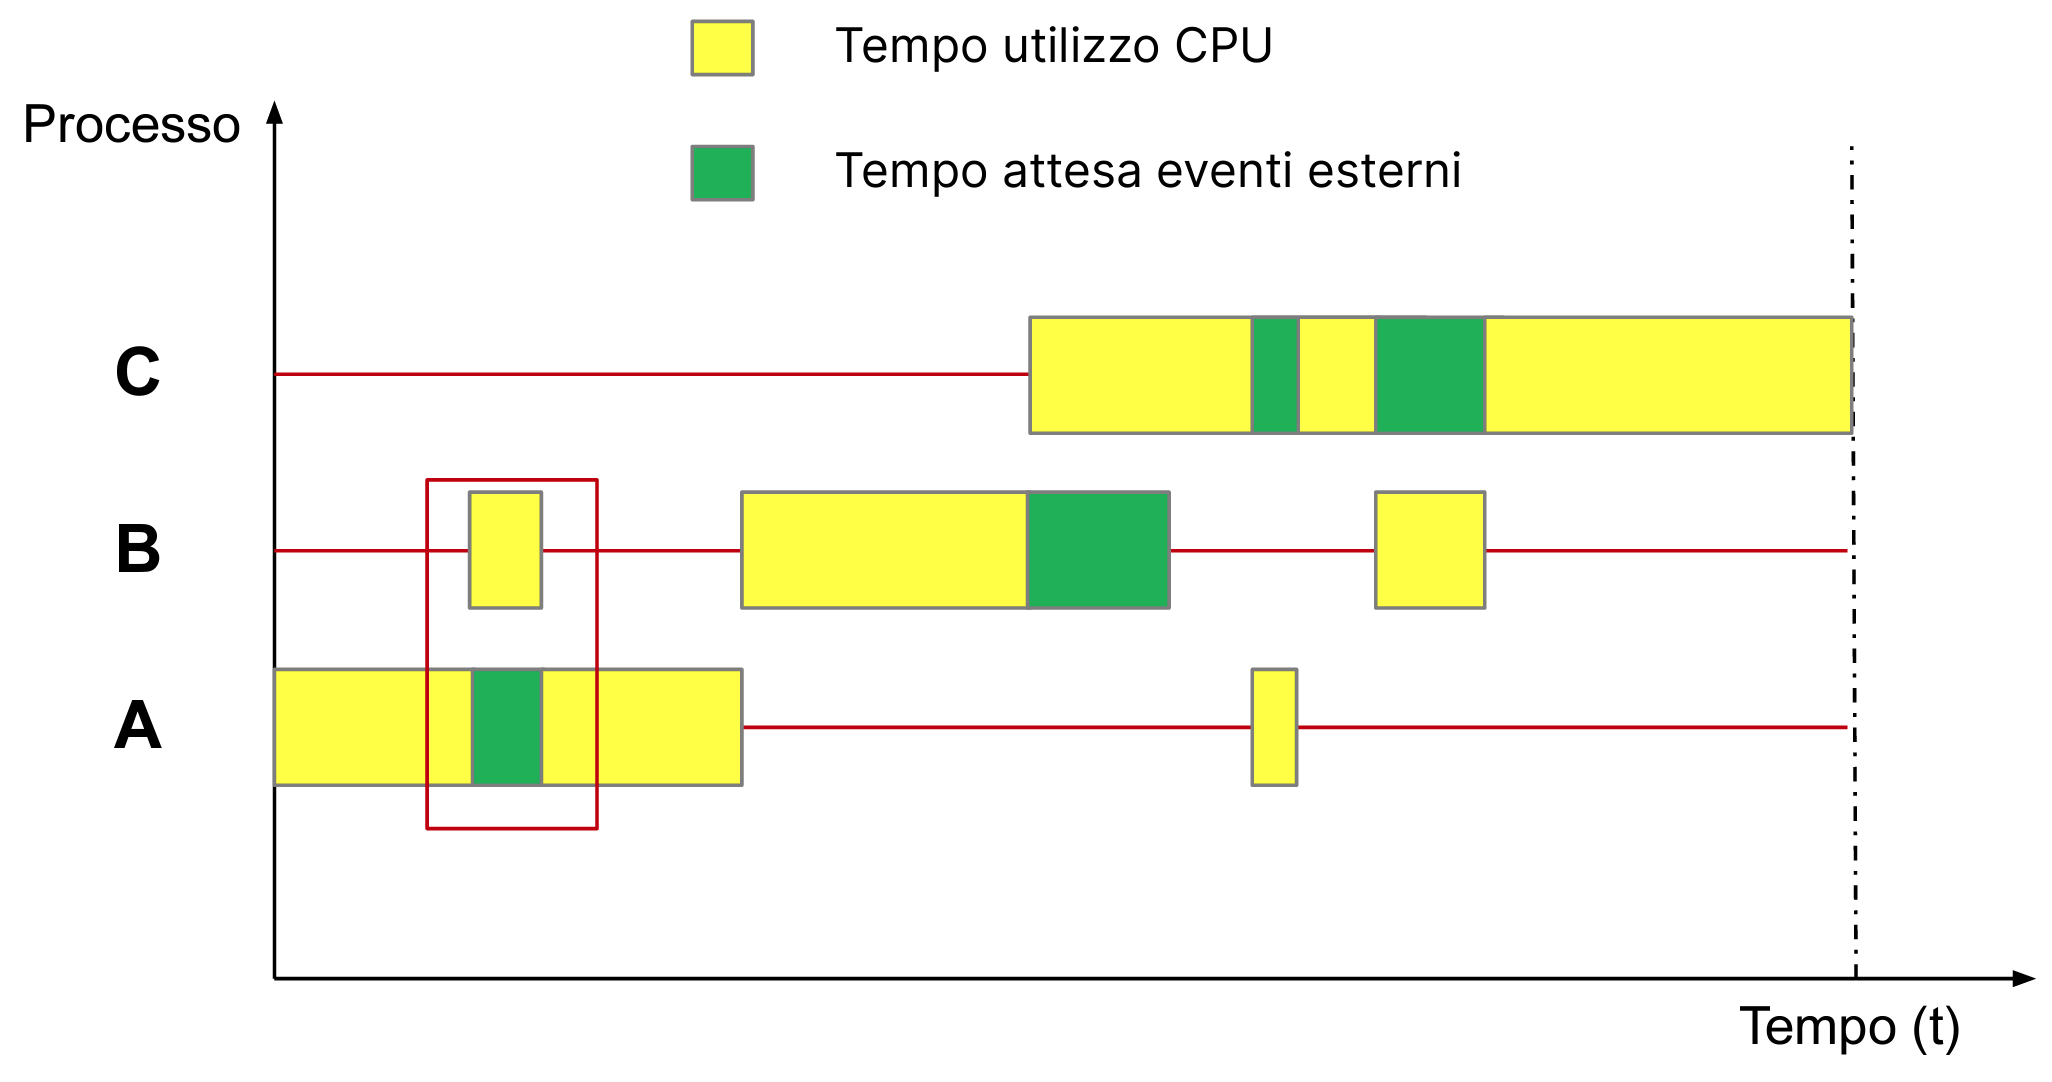
\includegraphics[width=0.8\textwidth]{images/multitask.png}
    \caption{Efficiency of Multitasking Systems}
    \label{fig:multitasking_efficiency}
\end{figure}

\subsection{Time-Sharing Systems}
An evolution of multitasking systems is time-sharing systems. In a time-sharing system, each process is executed cyclically for small time intervals called "time slices" or "quanta". With a sufficiently fast CPU, a time-sharing system gives the impression of parallel process evolution.

\begin{figure}[h]
    \centering
    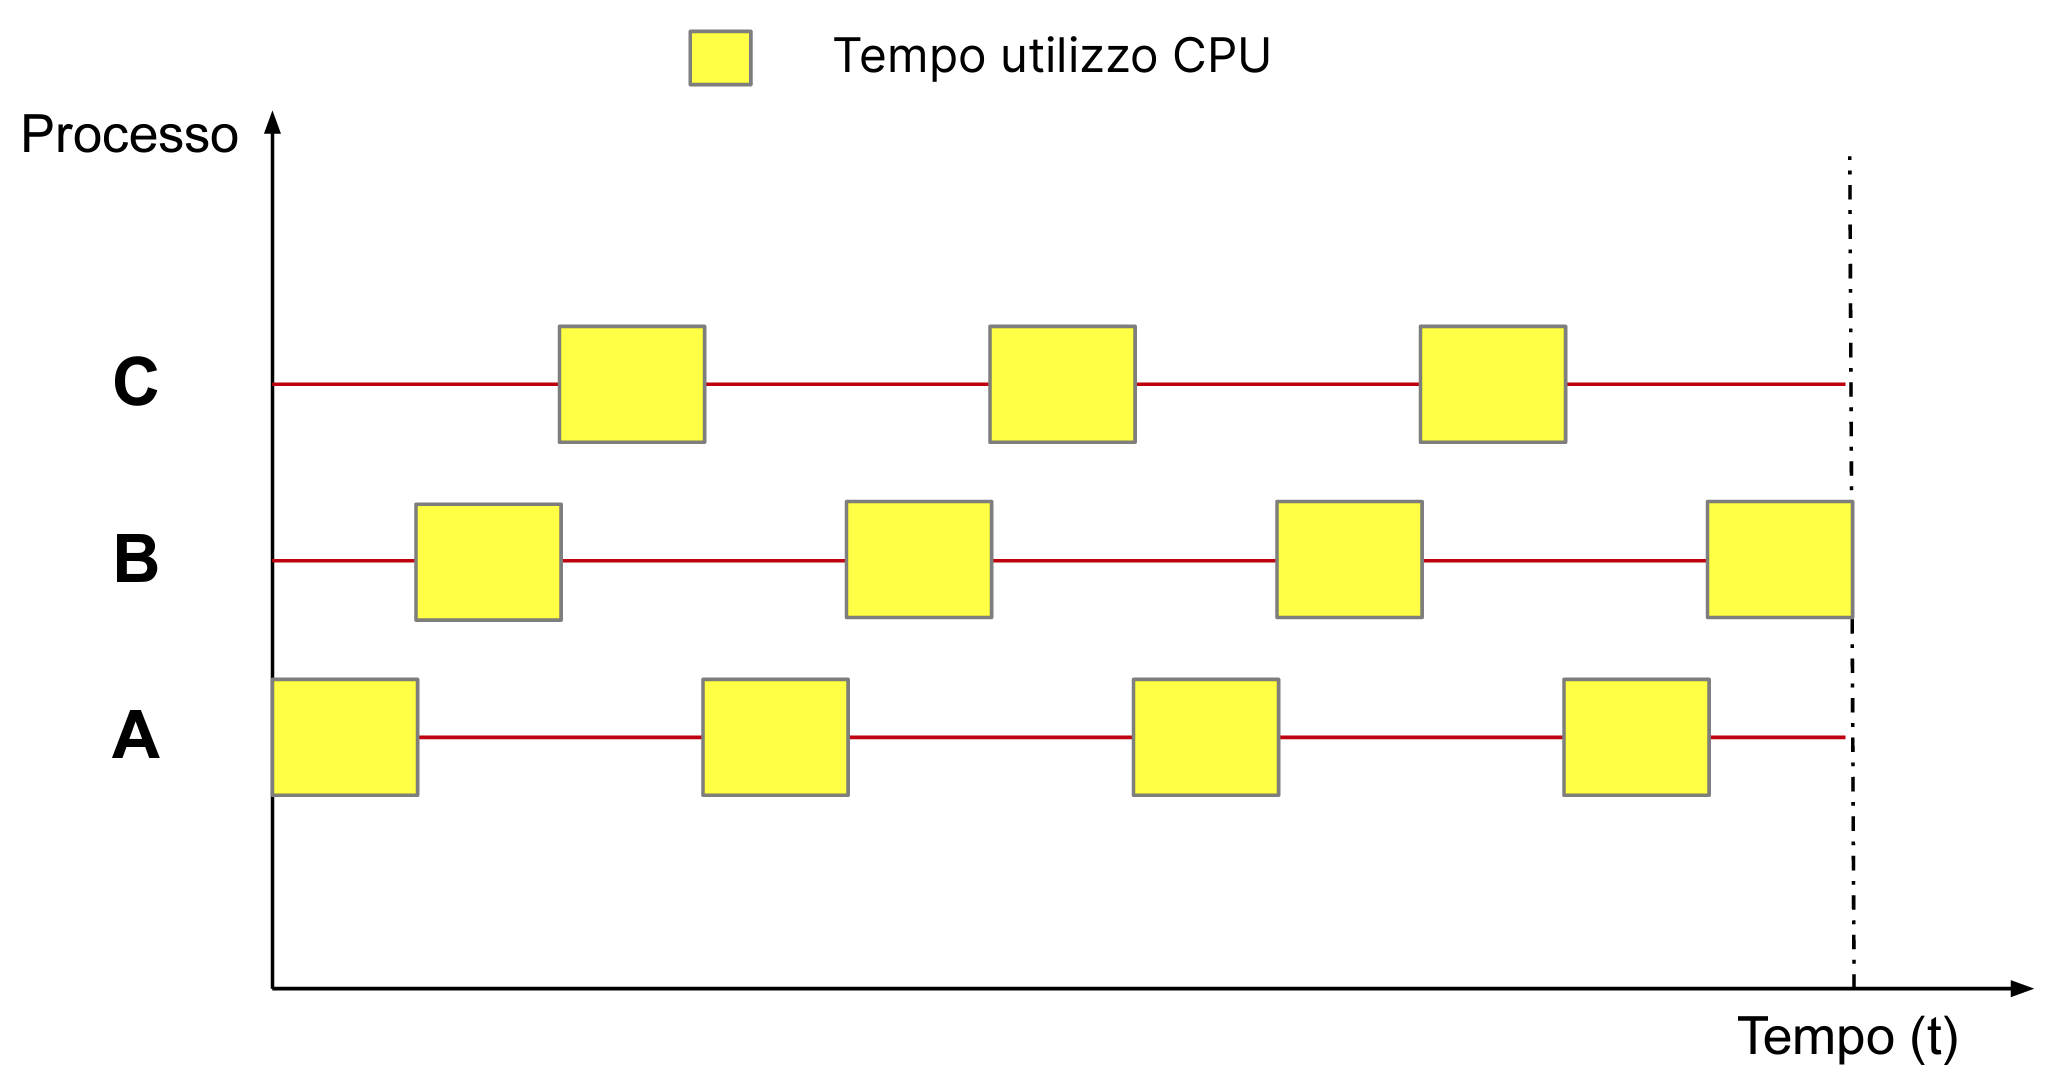
\includegraphics[width=0.8\textwidth]{images/timeshare.png}
    \caption{Time-Sharing System}
    \label{fig:time_sharing}
\end{figure}

In time-sharing systems, processes are executed for a standard period called a "quantum". The process is interrupted to execute another process for a "quantum", and so on.

\subsection{Preemptive and Cooperative Multitasking}
Common operating systems, such as Windows, macOS, and many Linux distributions, adopt preemptive multitasking to manage the simultaneous execution of multiple processes or applications. There are two main types of multitasking:

\begin{itemize}
    \item \textbf{Preemptive Multitasking}: In a preemptive multitasking system, the operating system allocates a certain period (time slice or quantum) to each process and then automatically switches to the next process. This approach is called "preemptive" because the operating system can interrupt a running process before it completes its execution period. This ensures fair distribution of system resources among processes.
    \item \textbf{Cooperative Multitasking}: In a cooperative multitasking system, it is the responsibility of individual processes to release control of the CPU when they no longer need it. This requires greater cooperation among processes, as they must be designed to voluntarily yield control. However, if a process does not release control, it can negatively impact system performance.
\end{itemize}

The operating system is a crucial software component that provides services to users and acts as an interface between the user and the physical machine. By managing hardware resources efficiently and providing a stable environment for applications, the operating system plays a vital role in the overall functionality and performance of a computer system.


\subsection{Memory Management in Operating Systems}
One of the central and most important tasks of an operating system is the management of central memory. But what is central memory? We can distinguish four types of central memory:

\begin{itemize}
    \item ROM (Read Only Memory): ROM is used by operating systems for computer initialization programs. Basic routines of computer systems, such as the BIOS (Basic Input/Output System), were traditionally written in ROM. Today, it is more accurate to refer to this type of memory as EEPROM.
    \item CPU Registers: CPU registers are very fast access memory locations used by the CPU to store instructions to be followed for short periods of time.
    \item Cache Memory: Cache memory represents areas where previously used data is temporarily stored for faster future access. Cache memories are quite limited and can only contain a small amount of data.
    \item RAM (Random Access Memory): RAM is the main memory of an operating system, and the greater the available amount, the better the PC's performance. RAM consists of a matrix of cells, each identified by an address in binary notation. When a process is executed by the CPU, its instructions, saved on secondary memory, must be loaded into RAM cells to be read.
\end{itemize}

Secondary memory, or mass memory, refers to non-volatile memory types (i.e., where information remains saved even when the machine is turned off). Examples include hard disks, USB flash drives, and SSDs.


\subsection{Memory Management Module}
The memory manager is the module responsible for allocating memory to various tasks when needed and removing tasks from memory when completed. The complexity of the memory manager is directly related to the type of operating system. In multi-tasking systems, managing multiple programs loaded in memory is more complex, particularly the optimal allocation of memory spaces.

\subsubsection{Linear Allocation Example}
Consider a multi-tasking system with three processes, A, B, and C.

\begin{enumerate}
    \item Process A transitions to the running state, and the CPU loads A's instructions into RAM.
    \item Next, it is B's turn, and the CPU loads B's instructions.
    \item The instructions of C are then loaded into memory.
\end{enumerate}

This model is known as linear allocation. The memory blocks occupied by each process depend on the number of instructions each process needs to execute.

\paragraph{Fragmentation Issue}
Consider the following scenario:
\begin{enumerate}
    \item Process C completes its work, and the CPU removes it from memory.
    \item Process D needs to be executed, but the memory space it requires is larger than what was freed by C. As a result, there will be unused free memory until a process that fits into the space freed by C can be found.
\end{enumerate}

\paragraph{Paging Solution}
The solution to the fragmentation problem is "paging." With this technique, memory is divided into blocks of equal size, called "pages." Each process that needs to be executed is allocated a portion of memory equal to one or more pages.

In this way, memory is used optimally, without free spaces.

\subsection{Virtual Memory}
There are situations where the memory is insufficient to hold all the processes. The concept of virtual memory is introduced, where the operating system creates what appears to be dedicated memory for each process. Only the necessary parts of code and data for the process are loaded into memory, while the rest is moved to a secondary memory area called the "swap area."

\begin{figure}[h]
    \centering
    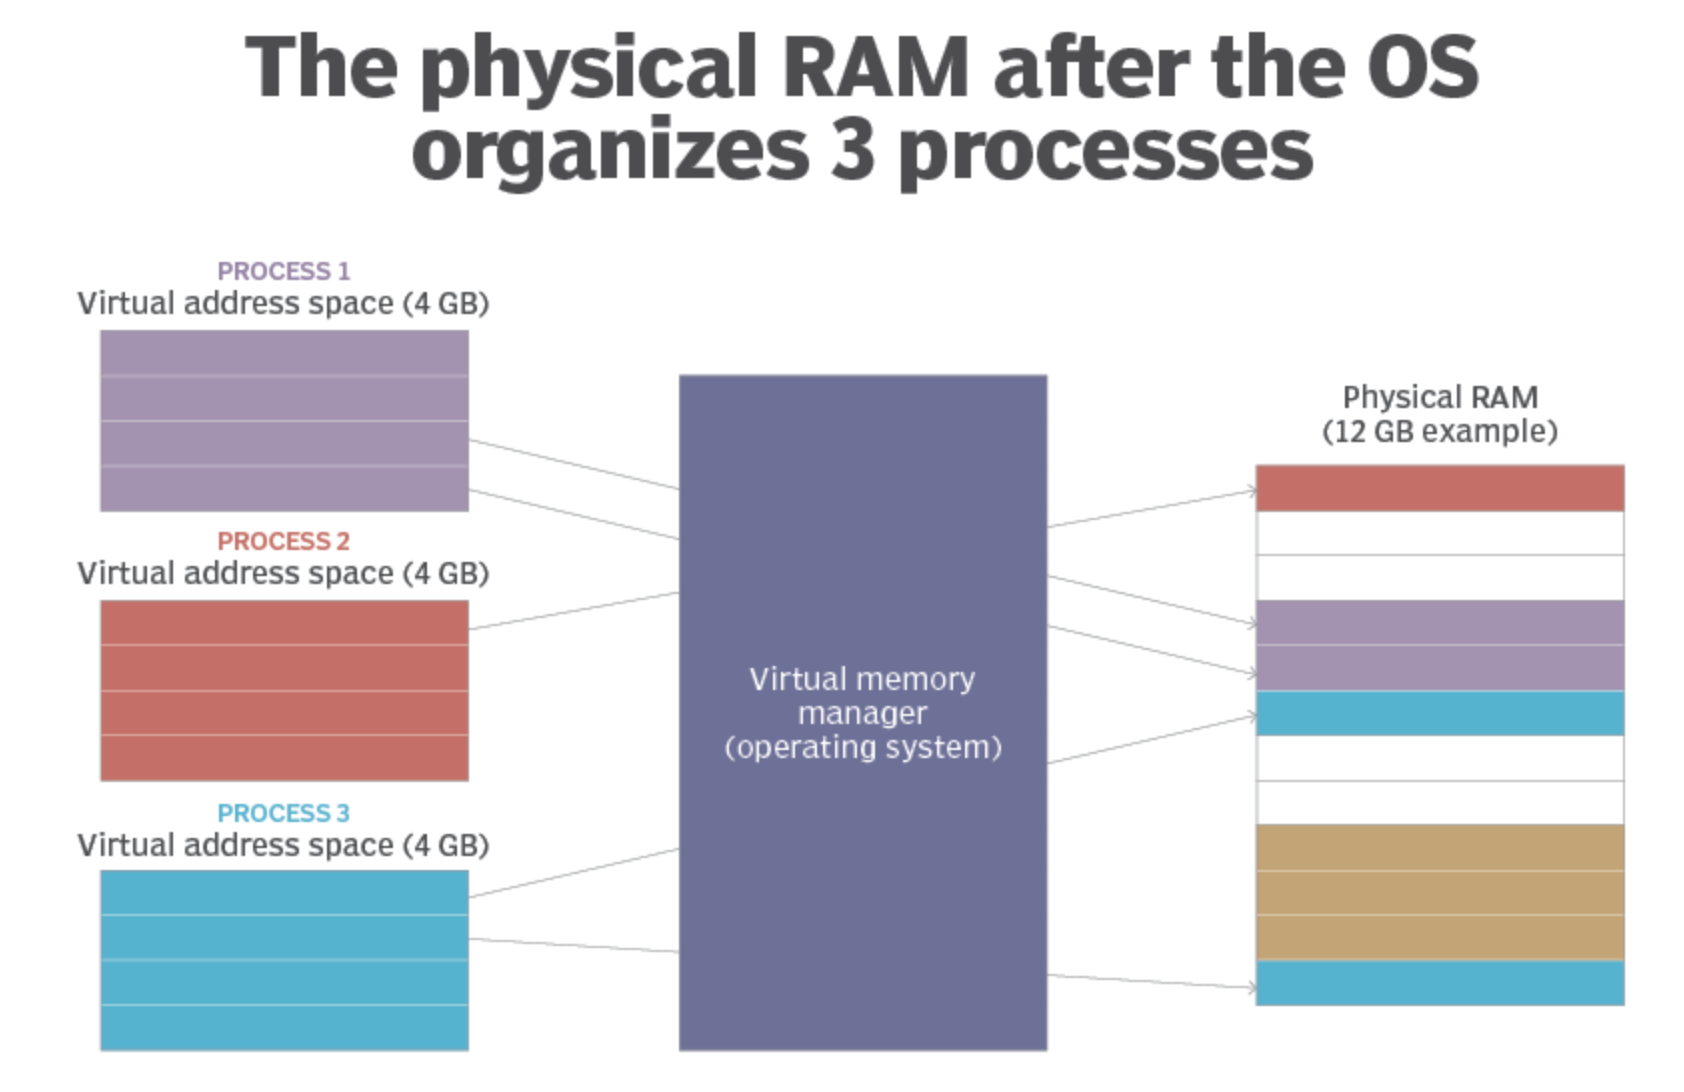
\includegraphics[width=0.8\textwidth]{images/memory.png}
    \caption{Virtual Memory Management}
    \label{fig:virtual_memory}
\end{figure}

The mehanisms for implementing virtual memory are complex, but modern processors have hardware mechanisms to facilitate its management.


Memory management is a critical function of an operating system, involving the efficient allocation and deallocation of memory resources to various processes. Techniques like paging and virtual memory help optimize memory usage and improve overall system performance, ensuring that the system can handle multiple tasks efficiently and effectively.

\subsection{File Systems in Operating Systems}
The file system manager is a module of the operating system responsible for managing information stored on secondary storage devices, also known as mass storage. Secondary storage refers to non-volatile memory, where stored data is permanent and does not depend on the state of the computer (on or off). The main role of the file system manager is to control and ensure the correctness and consistency of the information. Various technologies today offer different file systems to users, such as FAT32, NTFS, Apple File System, ext3, and ext4. Regardless of the technology, almost all file systems use a hierarchical approach, where directories are used to group multiple files together.

\subsubsection{Key Concepts of File Systems}
Here are some key concepts related to file systems:

\begin{itemize}
    \item File: a file is a logical unit of data containing information such as text, images, programs, or data.

    \item Directory (Folder): a directory is a logical container for files and other directories. Directories are organized in a tree structure, forming the hierarchy of a file system.

    \item Path: a path represents the location of a file or directory within the file system. For example, \texttt{C:\textbackslash Users\textbackslash username\textbackslash Documents} is a path in a Windows file system.

    \item Hierarchy: the directory structure forms a hierarchy that simplifies the organization of files in an orderly manner.
\end{itemize}

\paragraph{Types of File Systems}
There are various types of file systems, each with its own characteristics and uses. Some examples include NTFS (New Technology File System) and FAT32 on Windows systems, HFS+ on macOS, and ext4 on Linux systems.

\paragraph{Formatting}
Formatting a storage device creates a file system on it, preparing it for use. Formatting can affect the type of file system used.

\paragraph{Access and Security}
File systems often handle access control and data security, defining who can read, write, or execute certain files or directories.

In summary, the file system is a crucial component of any operating system, providing an organizational structure for efficiently storing and retrieving data.

\subsection{I/O Device Manager}
The Input/Output (I/O) device manager is a module of the operating system responsible for allocating devices to processes that request access, such as the mouse, keyboard, screen, and so on. To do this, the I/O device manager relies on software called "drivers" (you may have heard the term: "you need to download/update drivers for video cards, for example"), which are generally released by device manufacturers.

\subsubsection{Driver Functions}
Some main tasks performed by a driver include:

\begin{itemize}
    \item Managing signals to external peripherals (screens, keyboards, mice, etc.).
    \item Handling conflicts and synchronization when two processes need the same device simultaneously.
\end{itemize}

When a process requests access to an I/O device, the driver checks its status. If it is available, it assigns it to the process and marks the device as "busy." This way, synchronization problems between processes that request the same device simultaneously are avoided.

\subsection{User Experience}
One of the primary goals of operating systems is to support users and facilitate their tasks. All operating systems implement mechanisms to make the "user experience" easier, i.e., the use of the system by users. The user interface is what simplifies the interaction between users and hardware systems. Two categories of user interfaces can be distinguished:

\subsubsection{Textual User Interface}
Examples include command interpreters on Linux (shell) or PowerShell on Windows.

\subsubsection{Graphical User Interface}
The program outputs are displayed on the screen within windows.

The file system manager, I/O device manager, and user interface are crucial components of any operating system. They work together to provide an efficient, secure, and user-friendly environment for managing hardware resources and data. By understanding these components, we can appreciate the complex orchestration that allows modern operating systems to function seamlessly.

\subsection{Security in Operating Systems}

When discussing operating system security, it is essential to consider the external environment in which the system operates to determine appropriate security measures. A server running a critical application in a server room will certainly need physical security policies, such as being housed in a locked room with surveillance mechanisms. In contrast, a personal computer does not require a server room but must be protected from threats such as:

\begin{itemize}
    \item Unauthorized access
    \item Data modification or deletion
    \item Theft of confidential information
\end{itemize}


\subsubsection{Authentication}
Authentication is a process aimed at recognizing the user on a computer system. Generally, authentication is verified through login mechanisms that use credentials, which can be public like the username and secret like the password. To enhance the security of the login process, passwords are often subject to password security policies, which include a series of requirements, such as:

\begin{itemize}
    \item Password length: at least 8 characters
    \item Password complexity: at least one uppercase letter, one number, one symbol
    \item Password rarity: avoiding common passwords like \texttt{Password1!} or repeated characters
    \item Periodic password change: for example, every 3 months
\end{itemize}

In the authentication process, two main actors are involved:

\begin{itemize}
    \item The user who enters the credentials
    \item The authentication system, which verifies the credentials provided by the user
\end{itemize}

An authentication system verifies the user by comparing the credentials entered by the user with the credentials stored in a dedicated directory used to store data for all users who have access to the system, known as the \textit{user repository}.

There are two critical security aspects to consider in this process:

\begin{itemize}
    \item Credentials in the user repository must be stored encrypted, not in plaintext.
    \item Credentials in transit at points 2 and 3 should be either encrypted or transmitted over a secure channel.
\end{itemize}

Ensuring that data is encrypted both in transit between systems and when stored statically on a system is fundamental.

\subsubsection{Basic Authentication}
The example above illustrates basic authentication, as it uses only one step of authentication. For more sensitive applications, additional authentication methods can be added to provide an extra layer of security. Nowadays, the use of passwords alone is highly discouraged, and Multi-Factor Authentication (MFA) is strongly recommended. A second authentication factor, in addition to the password, could be one of the following:

\begin{itemize}
    \item \textbf{Something the user has}: e.g., a phone for authentication via push notification, app, or QR code.
    \item \textbf{Something the user knows}: e.g., a second factor such as a PIN.
    \item \textbf{Something the user is}: e.g., a second factor such as a physical characteristic, like facial recognition or fingerprint.
\end{itemize}

\subsubsection{Examples of Second Authentication Factors}
The use of a second authentication factor significantly enhances security because an attacker would need both your password and your second authentication method. Examples include Google and Microsoft Authenticator apps, which provide one-time codes, and banking apps that require a second authentication step for transactions.

\begin{table}[h]
    \centering
    \begin{tabular}{|l|l|}
    \hline
    \textbf{Second Factor} & \textbf{Description} \\ \hline
    Push notification – mobile app & The user receives a one-time code on a smartphone app \\ \hline
    USB Token & A hardware device generating a unique code \\ \hline
    Fingerprint/Facial recognition & Physical characteristic used as a second factor \\ \hline
    Phone call & The user receives a call with a numerical code \\ \hline
    \end{tabular}
    \caption{Examples of Second Authentication Factors}
    \label{tab:second_authentication_factors}
\end{table}


\subsubsection{Authorization}
While authentication handles user verification, authorization manages the privileges of a verified user. Authorization defines access rights to resources, such as read/write permissions on a file or executing a specific task. It is important to note that authorization follows authentication; once the user is verified, they are granted or denied permission to perform certain functions based on their privileges.

\paragraph{Access Control Models}
Authorization can be defined at the operating system level using one of the following models:

\begin{itemize}
    \item \textbf{Discretionary Access Control (DAC)}: Uses a decentralized model where the owner of a document can manage its privileges.
    \item \textbf{Mandatory Access Control (MAC)}: Uses a centralized model, assigning security labels to resources to classify information and specify authorized user groups.
    \item \textbf{Role-Based Access Control (RBAC)}: Assigns privileges based on user roles, adhering to the principle of least privilege.
\end{itemize}

\subsubsection{Accounting}
Accounting allows tracking of resource usage by a user. An example of accounting is system logs, which track events such as logins, logouts, and configuration changes for each user accessing the system. Given that most attacks on companies originate from internal users, accounting is crucial for identifying the perpetrators of malicious activities. For example, if your account is compromised through phishing, logs can trace all malicious activities performed with your account and possibly even the attempt to steal your credentials, thus protecting you from being held responsible.

Security in operating systems encompasses various aspects, including physical security, authentication, authorization, and accounting. By understanding and implementing these security measures, we can ensure a robust defense against both external and internal threats, providing a secure and reliable environment for users and applications.
